\section{Validation et performances}

L'objectif de cette section vise à proposer une méthodologie pour vérifier que l'implémentation de la structure de données offres de bonnes performances. Les études de performances menées dans cette section sont appliquées à l'implémentation à base de tableaux simples détaillées dans les sections précédentes, mais peuvent aussi s'appliquer à toute autre implémentation ultérieure.

\subsection{Performance des parcours}

Le but de cette section est de vérifier que la structure de données permet de parcourir les objets en utilisant au mieux les capacités de la machine. 

\subsubsection{Le benchmark}

Afin de mesurer la performance des parcours, un benchmark permettant de mesurer les temps d'exécution de différents parcours dans différentes situation a été mis en place.

\paragraph{Paramètres}

Le temps d'exécution d'un parcours est mesuré en faisant varier plusieurs paramètres :
\begin{itemize}
	\item $S$ : La taille des données à parcourir;
	\item I : L'intensité arithmétique, c'est à dire le nombre d'opération effectuées pour chaque objet;
	\item $N_{mpi}$ : Le nombre de processus MPI;
	\item $N_{threads}$ : Le nombre de threads OpenMP
\end{itemize}

\paragraph{Parcours testés}

La mesure est effectuée sur les parcours présentés en section \ref{sec:parcours}, ainsi que sur un parcours témoin :
\begin{itemize}
	\item Parcours des nœuds;
	\item Parcours des segments avec nœuds connectés;
	\item Parcours des nœuds avec segments connectés;
	\item 'Stream' sur des tableaux simples
\end{itemize}

\paragraph{Données}

Les données à parcourir sont générées en fonction de la taille demandée. Le réseau de dislocations généré se compose de $S/4$ boucles carrées uniformément réparties et composées de 4 segments, comme illustré dans la figure \ref{fig:testcase-bench-mesh}. La taille des boucles est modifiée en fonction du nombre de segments pour maintenir une densité de dislocations constante.

\begin{figure}
	\centering
	\begin{subfigure}{0.4\textwidth}
		\centering
		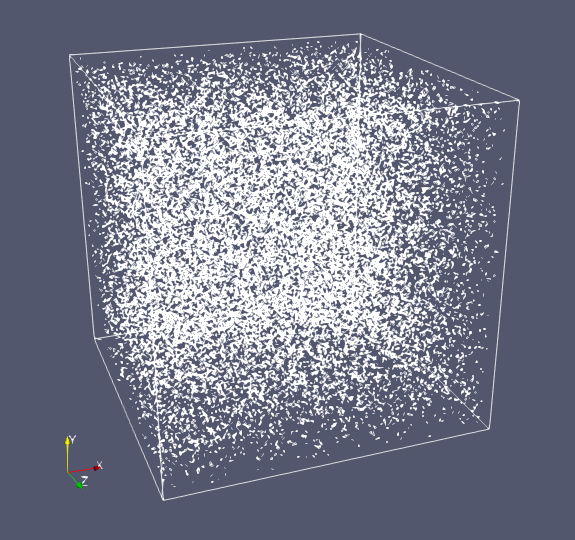
\includegraphics[width=\linewidth]{img/testcase-bench-mesh-1E5}
		\caption{$10^5$ Segments de taille $\unit{50}{\angstrom}$}
		\label{fig:testcase-bench-mesh-1E5}
	\end{subfigure}
	\begin{subfigure}{0.4\textwidth}
		\centering
		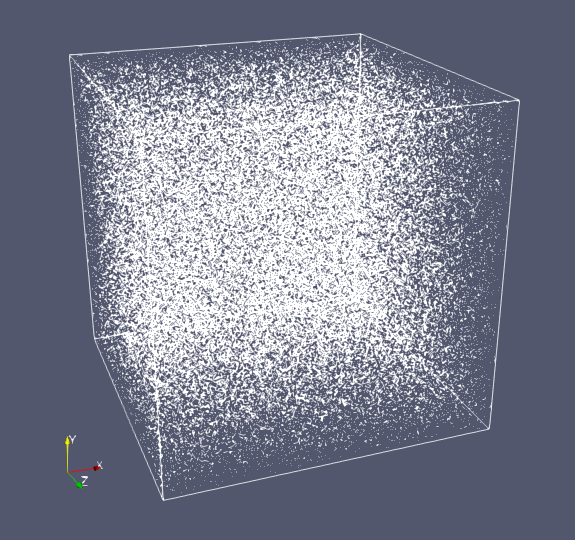
\includegraphics[width=\linewidth]{img/testcase-bench-mesh-1E6}
		\caption{$10^6$ Segments de taille $\unit{5}{\angstrom}$}
		\label{fig:testcase-bench-mesh-1E6}
	\end{subfigure}	
	\caption{Données générées pour tester la performance des parcours de la structure de données. Taille de domaine :\unit{1}{\micro\meter}; densité : $\unit{5\cdot 10^{14}}{\meter\per\meter\cubed}$ }
	\label{fig:testcase-bench-mesh}
\end{figure}

Pour le parcours témoin 'Stream', des tableaux de vecteurs à 3 dimensions de taille $S$ sont générés.

\paragraph{Opérations effectuées pour chaque objet}

Pour chaque élément contenu dans la structure de données, on effectue un certain nombre d'opérations en fonction de l'intensité arithmétique $I$ demandée. La fonction exécutée pour chaque objet est décrite dans l'algorithme \ref{algo:function-bench-mesh}. 

\begin{algorithm}[H]
	\SetAlgoLined
	\LinesNumbered
	\SetAlgoNoEnd	
	\DontPrintSemicolon
	\SetKwInput{KwParams}{Paramètres}
	\KwParams{$I$ : L'intensité arithmétique}
	\KwData{$v_1$, $v_2$ et $v_3$ : des champs vectoriels de la structure de données.}
	
	$v_1 \leftarrow 0$\;
	\For{ $i$ dans $[1,I]$ }
	{
		$v_1 \leftarrow v_1 + (0.1 \cdot i )\cdot v_2 + (0.15 \cdot i) \cdot v_3$\;
	}
	
	\caption{Fonction exécutée pour chaque objet}
\end{algorithm}

La boucle for est en réalité implémentée en utilisant les templates afin que le compilateur puisse appliquer toutes les optimisations possibles. les $(0.1 \cdot i)$ et $(0.15 \cdot i)$ sont donc des constantes flottantes connues à la compilation différentes pour chaque multiplication. Cela permet de s'assurer que le compilateur ne factorise pas les multiplications, et effectue bien le nombre d'opérations flottantes attendu.

$v_1$, $v_2$ et $v_3$ sont des vecteurs en 3 dimensions en double précision. Pour chaque objet, 9 flottants doubles précisions (8 octets) sont chargés ou écrits. Le nombre d'octets écrits ou chargés au cours du parcours est:
\begin{equation}
	M(I,S) = 72 \cdot S
\end{equation}

Pour chaque objet, et pour chaque tour de boucle, on effectue 2 additions et 2 multiplications. Le nombre d'opérations flottantes au cours d'un parcours est le suivant:
\begin{equation}
	Flops(I,S) = 4 \cdot I \cdot S
\end{equation}

L'intensité en Flops/Octets en fonction de $I$ est :
\begin{equation}
	Intensite(I) = \frac{1}{18} \cdot I
\end{equation}

Selon les parcours considérés, les champs choisis pour $v_1$, $v_2$ et $v_3$ varient. 

\begin{table}
	\begin{tabulary}{1.0\textwidth}{r||c|C|C}
		\textbf{Parcours} & $\bm{v_1}$ & $\bm{v_2}$ & $\bm{v_3}$\\
		\hline
		\hline
		Référence & Tableau 1 & Tableau 2 & Tableau 3 \\
		\hline
		Nœuds seuls & Nouvelle position & Ancienne position & Vitesse\\
		\hline
		Segments avec Nœuds & Force sur le segment & Force nodale nœud 1 & Force nodale nœud 2\\
		\hline
		Nœuds avec Segments & Force nodale & Force sur le $1^{er}$ segment connecté & Force sur le  $2^{eme}$ segment connecté\\
	\end{tabulary}
	\caption{ Champs choisis pour le benchmark des parcours }
\end{table}

\paragraph{Méthode de mesure du temps d'exécution}

La mesure du temps d'exécution des parcours de la structure de données se fait en utilisant des timers à grain fin à l'intérieur du code. La mesure retenue est le temps mesuré le plus court entre le début et la fin du parcours sur un échantillon de 100 parcours identiques. Cette mesure semble fiable, car elle est comparable à la moyenne des temps mesurés sur les 99 itérations, en omettant la $1^{ere}$ mesure (effets de cache). Cette méthode de mesure est inspirée du benchmark Stream \footnote{benchmark stream}.

\subsubsection{Mémoire partagée.}

Cette section s'intéresse à la performance de la structure de données en mémoire partagée avec OpenMP. Nous proposons une méthode pour vérifier que la structure de données utilise correctement le matériel dans un contexte multithreadé sur un seul nœud de calcul. 

\paragraph{Roofline Model et Machine de test}

Le roofline model est une représentation graphique de la performance d'une application. Il permet de comparer la puissance théorique du matériel à la vitesse d'exécution de l'application\footnote{ref roofline}. La courbe tracée représente la performance en Flops\per\second en fonction de l'intensité arithmétique en Flops\per Octet. Le graphique se décompose en deux parties:
\begin{itemize}
	\item La performance maximale du matériel. Elle peut être mesurée ou déduite des spécifications constructeur.
	\item Les mesures de performances de l'application.
\end{itemize}

La machine utilisée pour effectuer les mesures est le cluster de la Maison de la Simulation : Poincare\footnote{ref poincare}. La topologie d'un noeud de la machine est donnée par la figure \ref{fig:lstopo-poincare}.

\begin{figure}
	\centering
	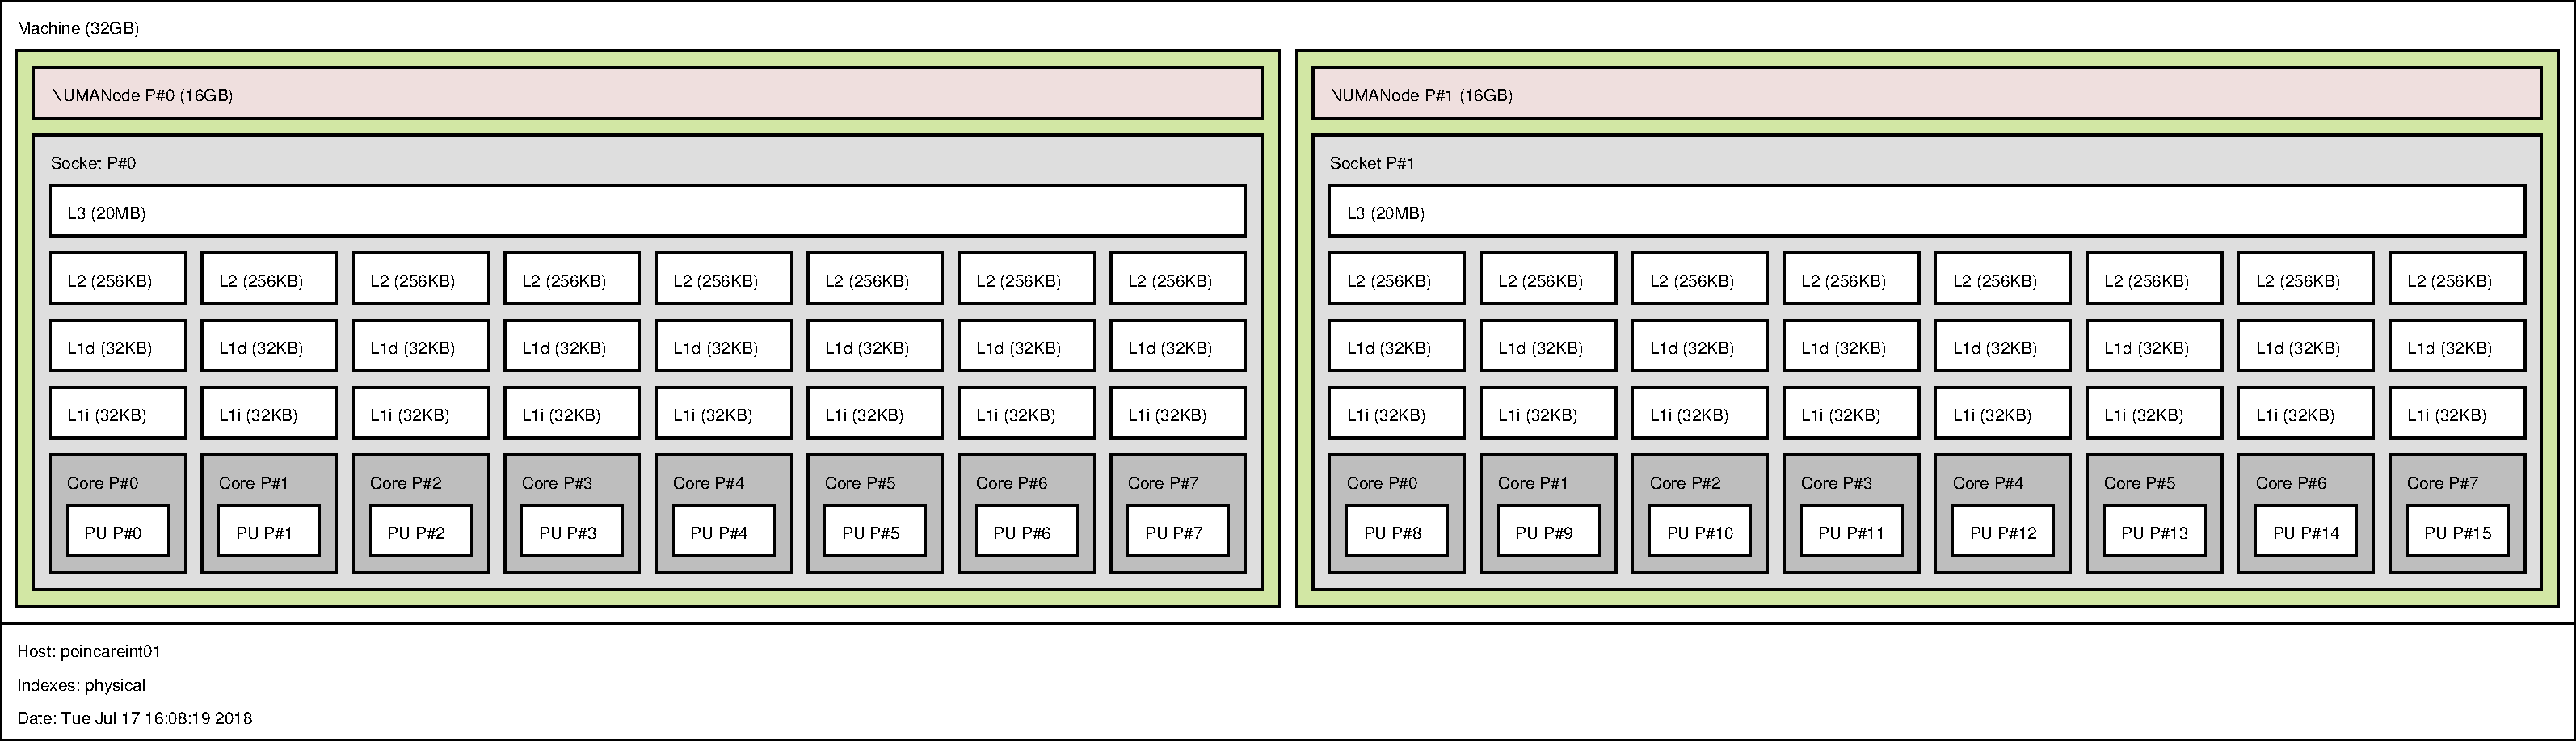
\includegraphics[width=\textwidth]{img/lstopo_poincare}
	\caption{Topologie d'un nœud de la machine Poincare}
	\label{fig:roofline_poincare}
\end{figure}

La performance maximale d'un nœud de la machine Poincare est résumée dans les roofline models de la figure \ref{fig:roofline_poincare}. 

\begin{figure}
	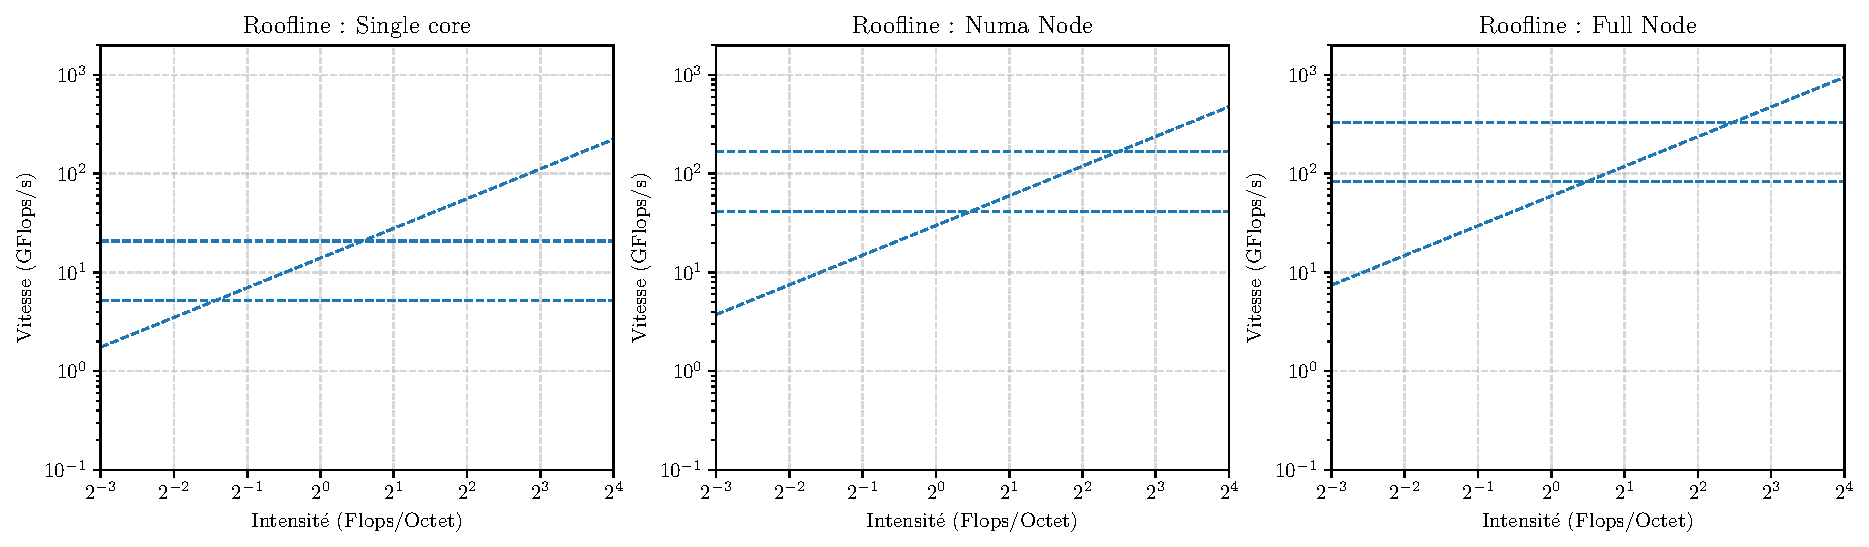
\includegraphics[width=\textwidth]{img/bench_mesh_roofline_limits}
	\caption{Performances de référence de la machine Poincare}
	\label{fig:roofline_poincare}
\end{figure}

Les 3 figures représentent les performances maximales de la machine avec différents nombre de threads:
\begin{itemize}
	\item 1 Thread
	\item 1 Noeud NUMA : 8 threads contraints sur un des deux nœuds NUMA en utilisant \texttt{numactl}
	\item Noeud de calcul complet : 16 threads
\end{itemize}

La bande passante maximale (partie linéaire) à été mesurée en utilisant le benchmark Stream, et la performance crête (plateau) a été déduite des spécifications constructeur du processeur:
\begin{align}
	P_{AVX2} &=& \unit{2.6}{\giga\hertz} \times \unit{2}{ALUs} \times \unit{4}{double\per inst} &=& \unit{20.8}{GFlops\per\second\per coeur}\\
	P_{scalaire} &=& \unit{2.6}{\giga\hertz} \times \unit{2}{ALUs} \times \unit{1}{double\per inst} &=& \unit{5.2}{GFlops\per\second\per coeur}
\end{align}
Le tableau \ref{tab:perf_poincare} résume les performances maximales de la machine.

\begin{table}
	\begin{tabulary}{1.0\textwidth}{R||c|c|c}
		 & 1 coeur & 1 NUMA & Noeud complet\\
		\hline
		\hline
		Bande Passante ( \giga O\per\second ) & 14.0 & 29.9 & 59.5 \\
		Performance crête scalaire (\giga Flops\per\second) & 5.2 & 41.6 & 83.2 \\
		Performance crête AVX2 (\giga Flops\per\second)  & 20.8 & 166.4 & 332.8 \\
	\end{tabulary}
	\caption{ Performances maximales de la machine. }
	\label{tab:perf_poincare}
\end{table}








\subsubsection{Environnement MPI}

\subsection{Performance des opérations topologiques}